%-------------------- begin preamble ----------------------

\documentclass
[twocolumn,
secnumarabic,
nobibnotes,
aps,
prl,
reprint,
groupedaddress,
amsmath,
amssymb,
]{revtex4-2}
\usepackage[caption=false]{subfig}
\usepackage{relsize,makeidx,color,setspace,amsfonts}
\usepackage{mathtools}


\usepackage{listings}
\lstset{
    language=Python,
    inputencoding=utf8,
    extendedchars=true,
    literate={ø}{{\o}}1 {å}{{\r a}}1 {Å}{{\r A}}1 {æ}{{\ae}}1,
    backgroundcolor=\color{white},
    basicstyle=\footnotesize\ttfamily,
    breakatwhitespace=false,
    breaklines=true,
    captionpos=b,
    commentstyle=\itshape\color{purple!60!black},
    frame=single,
    %identifierstyle=\color{orange},
    keepspaces=true,
    keywordstyle=\bfseries\color{violet},
    numbers=left,
    numbersep=5pt,
    numberstyle=\tiny\color{black},
    rulecolor=\color{black},
    showstringspaces=false,
    showtabs=false,
    stepnumber=1,
    stringstyle=\color{purple!60!black},
    tabsize=2,
    title=\lstname
  }
\usepackage{dcolumn}% Align table columns on decimal point
\usepackage[table]{xcolor}
\usepackage{bm,ltablex,microtype}
\usepackage{longtable}
\usepackage{siunitx}
\usepackage{algorithm2e}
\usepackage{csvsimple}
\usepackage{url}
\renewcommand{\UrlFont}{\small\tt}

\usepackage[pdftex]{graphicx}

\usepackage{fancyvrb} % packages needed for verbatim environments

\usepackage[T1]{fontenc}

\usepackage{ucs}
\usepackage[utf8]{inputenc}

\usepackage{neuralnetwork}

\usepackage{lmodern}         % Latin Modern fonts derived from Computer Modern

\usepackage{tikz}

% Hyperlinks in PDF:
\definecolor{linkcolor}{rgb}{0,0,0}
\definecolor{urlcolor}{rgb}{0,0,1}
\usepackage{hyperref}
\hypersetup{
breaklinks=true,
colorlinks=true,
linkcolor=linkcolor,
urlcolor=urlcolor,
citecolor=black,
filecolor=black,
%filecolor=blue,
pdfmenubar=true,
pdftoolbar=true,
bookmarksdepth=3   % Uncomment (and tweak) for PDF bookmarks with more levels than the TOC
}

\usepackage{csvsimple}
\usepackage{todonotes}
\setcounter{tocdepth}{2}  % levels in table of contents

% prevent orhpans and widows
\clubpenalty = 10000
\widowpenalty = 10000

% --- end of standard preamble for documents ---

% insert custom LaTeX commands...

\raggedbottom
\makeindex
\setlength{\textheight}{9.5in}


%-------------------- end preamble ----------------------

\begin{document}

% ------------------- main content ----------------------

\title{Time series forecasting using LSTMs\\Project 3 - FYS-STK4155}
\author{David Andreas Bordvik}
\email{davidabo@mail.uio.no}
\affiliation{Department of Informatics, University of Oslo}
\author{Gard Pavels Høivang}
\email{gardph@mail.uio.no}
\author{Are Frode Kvanum}
\email{afkvanum@mail.uio.no}
\affiliation{Department of Geoscience, University of Oslo}

\date{\today}

\begin{abstract}
  \begin{description}
  \item[Background] This part would describe the
  context needed to understand what the paper
  is about.
  \item[Purpose] This part would state the purpose
  of the present paper.
  \item[Method] This part describe the methods
  used in the paper.
  \item[Results] This part would summarize the
  results.
  \item[Conclusions] This part would state the
  conclusions of the paper.
  \end{description}
\end{abstract}

\maketitle

\section{Introduction}
The Norwegian and European power markets are changing. Several trends and demands in todays society result in increased electricity usage and power consumption. Additionally, a higher integrated fraction of renewable energy production coupled with tighter integration of power transmission infrastructure between countries affects several aspects within the power market, such as; electricity price, electricity production, electricity transmission, and electricity demand. A tighter connection of power infrastructure between countries also connects the power markets between countries to a greater extend, giving room for a growing number of market participants and competition. In the light of a changing and increasingly competitive power market, the need for forecasting the electricity price has become a fundamental process for energy companies. The ability to make qualitative decisions through forecasting the electricity price has never been more relevant. \cite{nowotarski_recent_2018}. Besides the aforementioned, studying the electricity price from a consumer standpoint considering the recent 
experienced extreme electricity price is the main motivation for this project. In this project, we focus on investigating the electricity price in the context of time-series analysis and forecasting the electricity price for the next day at an hourly resolution (24 hours). 
\\\\
There are five power regions in Norway named NO1, NO2, NO3, NO4, and NO5. Each region is a power market of its own, having its electricity price, and the regions can also be referred to as a bidding zone figure \ref{fig:biddin_zones}. The bidding name reflects the trading part, where participants buy and sell electricity. Each bidding zone has a day-ahead auction where electricity is traded for delivery the next day. In the day ahead market (the spot market), Nordpool finds the equilibrium between expected power demand and power production between aggregated quantities among all traders. Nord pool then sets the reference (system) price based on the equilibrium, sales, and purchase orders. The hourly electricity prices are then finalized for the next day, named day-ahead price or spot price. Nord pool closes the day-ahead market at 12:00 each day, and the hourly prices for the next day are published thereafter \cite{nordpool}. Even though the different zones are individual markets, they are still related to each other in many ways. All zones are interconnected via transmission cables, thus enabling power trading across bidding zones. All power markets and systems must be in balance at all times to ensure a stable and reliable power source. Therefore, power transmission is a major player affecting each power market's core, including the price. Another driver affecting the price is the cost of producing electricity. An increasingly integrating power production from renewable sources gives rise to new challenges since some renewable power sources are volatile in nature, e.g., wind power and solar. Having volatile power-producing contributors gives rise to added uncertainties to the electricity price. Therefore, highly accurate forecasting of the electricity price is regarded as very challenging considering the characteristics of the electricity price and the power markets \cite{li_day-ahead_2021, nogales_forecasting_2002,bunn_forecasting_2000}. Due to time constraints, this project only focuses on forecasting the electricity price for the bidding zone named NO2. 

\begin{figure}[t]
  \centering
  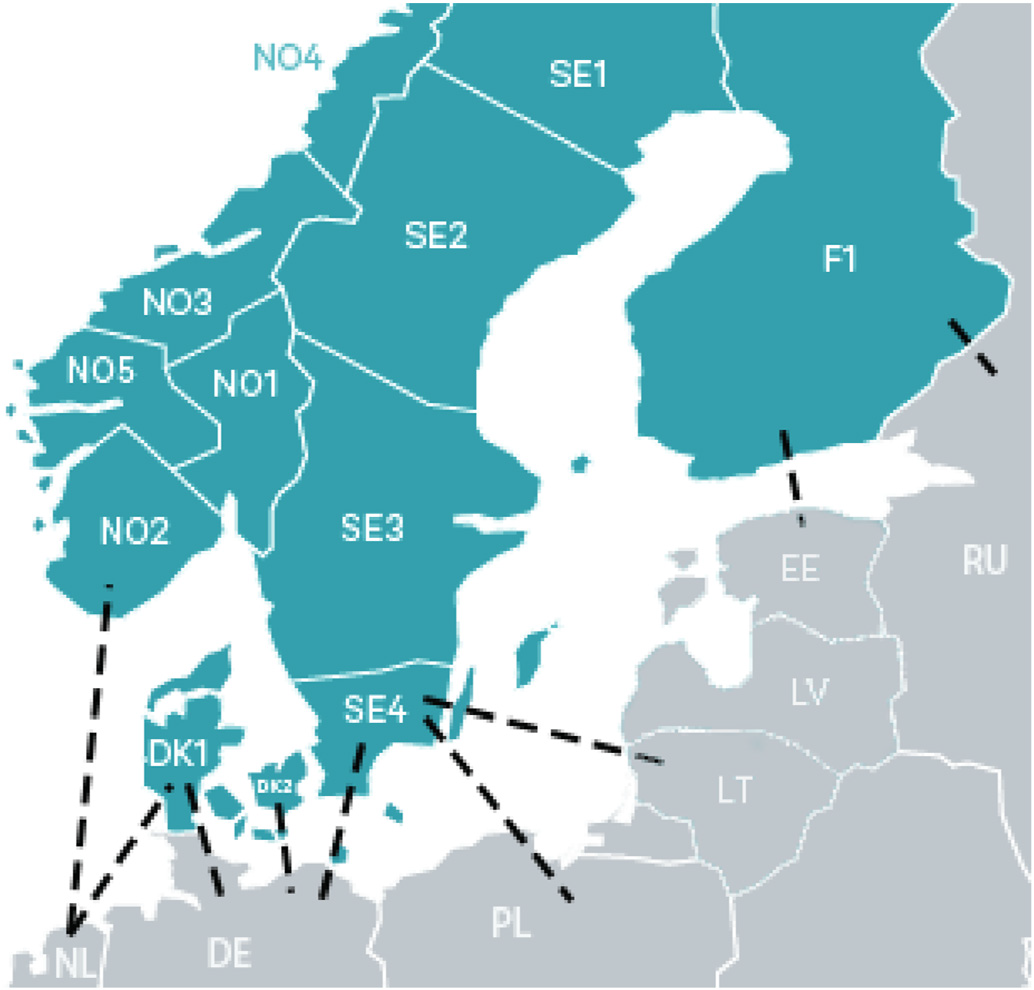
\includegraphics[width=90mm,scale=1.0]{figures/bidding_zones.png}
  \caption{Bidding zones - https://www.nordpoolgroup.com/the-power-market/Bidding-areas/}
  \label{fig:biddin_zones}
\end{figure}

In the two previous projects, we studied how spatial and time-independent data could be used to fit an arbitrary function with a given error following the Universal Approximation Theorem \cite{Nielsen2015} using a fully connected Neural Network. However, in Project 3, our data is sequential and time dependant. As such, a fully connected Neural Network is not designed to remember and make use of historical content while feeding foreward its current inputs. Therefore, this project will make us of Recurrent Neural Network and state-of-the-art methods for time-series data. A Recurrent Neural Network shares its weights across several time steps, which makes it suitble to use for temporal data \cite{Goodfellow2016}.


\section{Data}
The data used for this project is collected via tha Entsoe Transparnecy Platform API. \footnote{https://www.entsoe.eu/data/transparency-platform/}. We also look at "fyllingsgrad" over Norwegian dams, which represents potential power generation. The data is publicaly provided via The Norwegian Energy Regulatory Authority (NVE) \cite{noauthor_magasinstatistikk_nodate}. TESTTTTT


\subsection{Time series data}
\subsubsection{The nature of time series}
As already mentioned, in contrast to projects 1 and 2, this project deals with data in a sequential matter, called time series. What defines this type of format is that the data points decrease, increase or change in chronological order throughout time\cite{Vishwas2020 }.  A formal definition could be formulated as a mapping from a time-domain to real numbers:


\begin{equation}
  x: T \rightarrow  {\rm I\!R}^k 
\end{equation}

where T $\subseteq {\rm I\!R}$ and k $\in \mathbb{N}$ \cite{Auffarth2021}


In the scope of this project, our time series consist of discrete values that describe how various aspects regarding the energy sector changes over time. 

Dealing with data on such a format might yield an additional complexity when trying to analyze the raw data at hand. 

\subsection{Structuring our data}
The dataset used for this project can be found in GitHub linked in the appendix, in the data folder. The file used is the aptly named MAIN\_DATASET.csv. The file contains 51649 rows and 20 columns containing variables related to power region 2 and 5 in Norway. The dataset has been preprocessed such that it does not contain any NaN values, \todo[inline]{MER OM PREPROC AV DATA}. When feeding data into the RNN, which will be described in greater detail in the coming sections, the data has to be formatted to take the form of the 3D array $\left(\text{Batch Size}, \text{Time Steps}, \text{Dimensionality}\right)$. Specifically, Batch Size refers to the number of samples, Time Steps is the total number of the input width added with the forecast horizon, and finally dimensionality refer to the number of time series used, such that dimensionality $= 1$ would refer to a univariate time series. 


\section{Theory and Methods}
\subsection{Data Windowing}
We have applied a window based algorithm to structure the data into appropriate sample sizes that fit the constraints imposed by the Recurrent Neural Network. In comparison to the previous projects, our data does not contain a relationship between some input data and some target variable, instead we want to recognize the relationship throughout a sequence of values. Before sectioning the data into windows, we note that our data is evenly spaced, in our case we have an hourly time series. 

Our window algorithm starts off by sectioning the data into 24-hour chunks. This allows some flexibility when specifying the input width in terms of a varying number of days. Secondly, a window of length input width and forecast horizon containing 24-hours large cells with a final cell the size of the forecast horizon strides through the chunks with a stride of $1$ day (in other words it moves one chunk at a time). This generates a consecutive sample from our data, which is then restructured together with the other generated consecutive samples to match the required 3D array format imposed by the Recurrent Neural Network.

Since the chunks containing days are repeated in all data windows within the range of the sliding window, we are able to reuse data points in new isolated sequences as the window strides though the chunks. This allows us to effectively increase the number of samples, as contiguous samples contain overlapping data, though differ with regards to the first day used in the input width and data used as forecast horizon. This data window structure allows us to forecast an arbitrarily amount of time ahead, based on the data from a specified number of days ago.

Finally, during train test split, a single data window sample is split in such a way that the input width defines our X (input signal), and the forecast horizon specifies labels y. If the labels y have a length of 1, the RNN is a sequence to vector model predicting a single time step ahead. However, a label vector y with length greater than 1 would not itself specify whether the Recurrent Neural Network is a vector or sequence outputting model, as that would have to be specified in the model declaration. However, a length greater than 1 would indeed indicate that the model is forecasting several time steps ahead. 




\subsection{Sequence processing using Recurrent Neural Networks}
As our data is sequenced over time, we need a Neural Network that can share its weights across time steps. In a Recurrent Neural Network, this is done by applying the same update rule to the previous output when producing a new output \cite{Goodfellow2016}. Mathematically, we can define this system as
\begin{equation}
  \nonumber
  \bm{s}^{(t)} = f(\bm{s}^{(t-1)},\bm{x}^{(t)};\bm{\theta})
\end{equation}
Where $\bm{s}^{(t)}$ is the state of the system, $\bm{x}^{(t)}$ is an external signal which drives the system and $\bm{\theta}$ parametrizes $f$, though we note that this system itself does not contain any output. 

Recurrent Neural Networks support multiple different input and output sequences \cite{Geron2019}. A tuple of inputs or outputs over different time steps is considered a sequence, whereas a input or output from a singular time step is considered a vector. RNNs support different constellations of sequence/vector input and output, such that it is possible to input a sequence and output a sequence where some time steps are ignored. This is a favorable property given our data and task of producing a full day forecast some time steps after the end of our input sequence.

\subsection{Backpropagation through time}
Though computing the gradient through a Recurrent Neural Network is analogous to how it was computed in a Feed Forward Neural Network, the algorithm has to be applied throughout all the time steps of the Recurrent Neural Network recursively. The recursion starts at the final time step, where at the final time step $\tau$ the gradient of the loss $L$ can be computed as follows, using the notation of \cite{Goodfellow2016}
\begin{equation}
  \nabla_{\bm{h}^{(\tau)}}L = \bm{V}^T \nabla_{\bm{o}^{(\tau)}}L
\end{equation}
where $\bm{V}$ is the weights between the hidden states and output values $\bm{o}$.
Going backwards trough time ($t < \tau)$, the gradient of the propagated loss can be computed using the following equation
\begin{equation}
  \bm{W}^TJ(\bm{a})(\nabla_{\bm{h}^{(t+1)}}L)+\bm{V}^T(\nabla_{\bm{o}^{(t)}}L)
\end{equation}
where $\bm{W}$ is the weights associated with the hidden-to-hidden state connection and $J(\bm{a})$ is the jacobian of the activation function.

Given a long time sequence, a Recurrent Neural Network can be both memory and cpu intensive. Moreover, for long sequences of data, the unrolled RNN will be a considerably deep Neural Network. As we discussed in Project 2, a deep Neural Network is prone to the unstable gradient problem, where the gradient can either completely vanish or explode through the bounds of the datatype used to contain the value. In addition to the RNN being prone to unstable gradients given a long sequence, the memory of the first inputs will deter if the RNN is processing a long sequence \cite{Geron2019}.

\subsection{The unstable gradient problem}
Our main motivation behind introducing different activation functions such as the ReLU and Leaky ReLU to replace the Sigmoid activation function in Project 2 was to avoid the vanishing gradient which arose from the bounded output from the Sigmoid. However, a non-saturated activation function such as the ReLU family of functions runs the risk of updating the set of weights between two layers in such a way that the computed output is slightly increased. For a Feed Forward Neural Network, given how additional sets of weights are computed during gradient descent, this weight update pattern is not given to reoccur. Though for a Recurrent Neural Network, the same sets of weights are updated at every time step, such that a weight update pattern that ends up in a slight increase of the output would be reapplied until the output explodes \cite{Geron2019}. As such, when implementing a Recurrent Neural Network in the coming Section, we will use a saturating activation function such as the Hyperbolic Tangent $\tanh = \frac{\sinh}{\cosh}$, which conveniently is supplied as the default activation function for RNNs in TensorFlow \cite{tensorflow2015-whitepaper}.

\subsection{The Short-Term memory problem}
The second problem which arises in the context of training a Recurrent Neural Network is its inevitable memory loss of the earliest states as a result of how some information is lost for each time step \cite{Geron2019}. By following the approach of \cite{Hochreiter1997}, implementing Long Short-Term Memory (LSTM) cells can alleviate the memory loss. The idea behind LSTM cells is to store some information in the long-term, while at the same time forget unnecessary information whilst reading the rest which result in the short term output memory. In this way, for each time step some information is kept, while at the same time some long term memories are dropped if they meet certain requirements after each time step \cite{Geron2019}. As such, LSTM cell can be able to recognize, preserve, utilize and abolish trends in the data as needed, acheiving a better mean squared error than for the simple RNN cell. 
Another gated RNN which might alleviate the short term memory problem of Recurrent Neural Networks is the Gated Recurrent Unit, which simplifies the LSTM cell by combining the forget and output gate into one single gate \cite{Goodfellow2016}. additionally, the GRU cell merges both the long term memory state and the hidden state into a single vector. Though a GRU cell would outperform an LSTM cell in terms of computational efficiency \cite{Geron2019}, GRU as well as other gated RNNs derived from the LSTM cell performs approximately the same as LSTM \cite{Greff2015}.
A long sequence can also be shortened by applying a 1-dimensional convolutional layer as a pre-processing layer, before passing the shortened signal on to an RNN. Given our current application, the convolutional layer will effectively downsample a given input sequence, given the size of the convolutional kernel \cite{Geron2019}. The convolutional layer will both detect structures in the sequence as well as shortening the sequence. This in turn can benefit the RNN in terms of its memory, as it will be able to remember longer sequences than in the absence of a preprocessing convolutional layer.
Another preprocessing layer which might improve the performance of a RNN is a FeedForward layer. The FeedForward layer will project the input into a feature space with temporal dynamics, which may yield improved performance. \cite{Murugan2018}

Throughout this project, we will study both the effect of the aforementioned architectural differences, namely the difference between a sequence to vector and sequence to sequence RNN when predicting several time steps ahead. Furthermore, we will also study the effect of the different preprocessing techniques outlined above in response to both the gradient and memory loss problem. All in context of the ENTSOE dataset. 

\subsection{Setting up our RNN}
What follows is the basic structure that our developed RNN models will attain, following the constraints and conditions outlined in the previous sections. For clarity, all RNNs will be developed using the Keras frontend of TensorFlow \cite{tensorflow2015-whitepaper}. For a complete implementation of the models, we refer to the GitHub linked in the Appendix. 

We have developed models that are able to forecast a single, as well as several time steps ahead in time both via a vector and sequence approach. The main difference between a sequence to vector and sequence to sequence in terms of the RNN architecture is how the final recurrent layer returns its output. For a sequence to vector model, the only the final output node is considered, whereas for a sequence to sequence model we set the \textit{return\_sequences} flag to \textbf{True} as that would return all computed output nodes distributed through time. Finally, regardless of model architecture, a regular Dense feed forward layer distributes the output of the Recurrent Layer according to the specified forecast Horizon. Note that a Dense layer in TensorFlow supports sequences as input, meaning that it can handle the output from a recurrent layer regardless of vector or sequence form \cite{Geron2019}. 

A preprocessing layers such as a 1-dimensional convolution layer or a FeedForward layer can be implemented akin to the layers discussed above, taking the place as the input layer for their specific model.

As stated previously, the hyperbolic tangent function is sufficient as activation function for an RNN due to its saturating property. As such, our RNNs will default to the hyperbolic tangent as activation function. Moreover, an adaptive learning rate optimizer during gradient descent is chosen. For our models, we will default to the ADAM optimizer.

\section{Results}

\section{Discussion}

\section{Conclusions}

\appendix

\section{Source Code}
\label{sec:sc}
Link to github repository containing all developed code for this project: \textbf{CORRECT URL HERE}%\url{https://github.com/AndreasBordvik/FYS-STK4155-Prj2_report}

% Create the reference section using BibTeX:

% ------------------- end of main content ---------------

\bibliographystyle{plain}
\bibliography{biblio}




\end{document}